\documentclass[
    25pt,
    a0paper,
    portrait,
    colspace=2cm,
    blockverticalspace=2cm
]{tikzposter}

% \usepackage{lmodern}
\usepackage{amsmath}
\usepackage{amssymb}
\usepackage{physics}
\usepackage{bm}
\usepackage{blindtext}

\usetikzlibrary{patterns}

% Turn off the tikzposter watermark
% \tikzposterlatexaffectionproofoff

%% THEMING
%%--------------------------------------------------
%% THEMING
%%--------------------------------------------------

%%--------------------------------------------------
%% FONTS
%%--------------------------------------------------
\usepackage{fontspec}
\usepackage{anyfontsize}
\usepackage[sfdefault]{FiraSans}
\usepackage[scaled=1.15]{newtxmath}

%&--------------------------------------------------
%& COLORS
%%--------------------------------------------------

%%% IBM Carbon colorscheme
%%% https://carbondesignsystem.com/guidelines/color/overview/
\definecolor{Foreground}{RGB}{22, 22, 22}
\definecolor{Background}{RGB}{244, 244, 244}
\definecolor{Blue100}{RGB}{0, 17, 65}
\definecolor{Blue90}{RGB}{0, 29, 108}
\definecolor{Blue80}{RGB}{0, 45, 156}
\definecolor{Blue70}{RGB}{0, 67, 206}
\definecolor{Blue60}{RGB}{15, 95, 254}
\definecolor{Blue50}{RGB}{69, 137, 255}
\definecolor{Blue40}{RGB}{120, 169, 255}
\definecolor{Blue30}{RGB}{166, 200, 255}
\definecolor{Blue20}{RGB}{208, 226, 255}
\definecolor{Blue10}{RGB}{237, 245, 255}
\definecolor{Red}{RGB}{218, 30, 40}
\definecolor{Orange}{RGB}{255, 131, 43}
\definecolor{Yellow}{RGB}{253, 220, 105}
\definecolor{Green}{RGB}{25, 128, 56}
\definecolor{Grey05}{RGB}{240, 240, 240}
\definecolor{Grey10}{RGB}{224, 224, 224}
\definecolor{Grey15}{RGB}{211, 211, 211}
\definecolor{Grey20}{RGB}{198, 198, 198}
\definecolor{Grey30}{RGB}{168, 168, 168}
\definecolor{Grey40}{RGB}{141, 141, 141}
\definecolor{Grey50}{RGB}{111, 111, 111}
\definecolor{Grey60}{RGB}{82, 82, 82}
\definecolor{Grey70}{RGB}{57, 57, 57}
\definecolor{Grey80}{RGB}{38, 38, 38}
\definecolor{Grey90}{RGB}{22, 22, 22}
\definecolor{White}{RGB}{255, 255, 255}
\definecolor{Black}{RGB}{0, 0, 0}

\definecolorstyle{MyColorStyle}{
    % Random colors
    \definecolor{colorOne}{named}{Blue70}
    \definecolor{colorTwo}{named}{Green}
    \definecolor{colorThree}{named}{Red}
}{
    % Background Colors
    \colorlet{backgroundcolor}{White}
    \colorlet{framecolor}{Grey50}
    % Title Colors
    \colorlet{titlefgcolor}{Background}
    \colorlet{titlebgcolor}{colorOne}
    % Block Colors
    \colorlet{blocktitlebgcolor}{Background}
    \colorlet{blocktitlefgcolor}{colorOne}
    \colorlet{blockbodybgcolor}{Background}
    \colorlet{blockbodyfgcolor}{Foreground}
    % Innerblock Colors
    \colorlet{innerblocktitlebgcolor}{Grey10}
    \colorlet{innerblocktitlefgcolor}{colorTwo}
    \colorlet{innerblockbodybgcolor}{Grey10}
    \colorlet{innerblockbodyfgcolor}{Foreground}
    % Note colors
    \colorlet{notefgcolor}{black}
    \colorlet{notebgcolor}{colorTwo!50!white}
    \colorlet{noteframecolor}{colorTwo}
}

\usecolorstyle{MyColorStyle}


%%--------------------------------------------------
%% BACKGROUND
%%--------------------------------------------------
\definebackgroundstyle{MyBackground}{
    \fill[
        backgroundcolor,
        inner sep=0pt,
        line width=0pt,
    ] (bottomleft) rectangle (topright);
}

\usebackgroundstyle{MyBackground}


%%--------------------------------------------------
%% BLOCKS
%%--------------------------------------------------
\defineblockstyle{MyBlockStyle}{
    titlewidthscale=1,
    bodywidthscale=1,
    titlecenter,
    titleoffsetx=0pt,
    titleoffsety=10pt,
    bodyoffsetx=0mm,
    bodyoffsety=15mm,
    bodyverticalshift=5mm,
    roundedcorners=0,
    linewidth=1pt,
    titleinnersep=1.2cm,
    bodyinnersep=1.2cm
}{
    \ifBlockHasTitle
        % Body
        \fill[
            blockbodybgcolor,
            rounded corners=\blockroundedcorners,
            line width=\blocklinewidth
        ] (blockbody.south west) rectangle (blockbody.north east);
        % Block Title
        \fill[
            fill=blockbodybgcolor,
            rounded corners=\blockroundedcorners,
            line width=\blocklinewidth
        ] (blocktitle.south west) rectangle (blocktitle.north east);
    \else
        % Only body
        \fill[
            blockbodybgcolor,
            rounded corners=\blockroundedcorners,
            line width=2\blocklinewidth
        ] (blockbody.south west) rectangle (blockbody.north east);
    \fi
}

\defineinnerblockstyle{MyInnerBlockStyle}{
    titlewidthscale=1,
    bodywidthscale=1,
    titleleft,
    titleoffsetx=0pt,
    titleoffsety=0pt,
    bodyoffsetx=0mm,
    bodyoffsety=0mm,
    bodyverticalshift=-10mm,
    roundedcorners=0,
    linewidth=1pt,
    titleinnersep=0.8cm,
    bodyinnersep=0.8cm
}{
    % Body
    \fill[
        innerblockbodybgcolor,
        rounded corners=0,
        line width=\innerblocklinewidth
    ] (innerblockbody.south west) rectangle (innerblockbody.north east);
    % Block Title
    \fill[
        innerblocktitlebgcolor,
        rounded corners=0,
        line width=\innerblocklinewidth
    ] (innerblocktitle.south west) rectangle (innerblocktitle.north east);
}

\useblockstyle{MyBlockStyle}
\useinnerblockstyle{MyInnerBlockStyle}
\newcommand{\myblock}[2]{\block{{\LARGE \bfseries \sffamily \addfontfeature{LetterSpace=3.0} #1}}{\large #2}}


%%--------------------------------------------------
%% TITLE
%%--------------------------------------------------
\definetitlestyle{MyTitle}{
    width=\textwidth,
    roundedcorners=0,
    linewidth=4pt,
    innersep=1.5cm,
    titletotopverticalspace=-1mm,
    titletoblockverticalspace=15mm
}{
    \begin{scope}[line width=\titlelinewidth]
        \fill[
            fill=Foreground
        ] (\titleposleft, \titleposbottom) rectangle (\titleposright, \titlepostop);
        \draw[color=titlebgcolor, line width=10, shorten <=-3pt, shorten >=-3pt]
            (\titleposleft, \titleposbottom) -- (\titleposright, \titleposbottom);
        \path (\titleposleft, \titlepostop) -- ++(0, -1) node [anchor=north west, inner sep=20pt] {\includegraphics[scale=1.2]{figures/unibo_neg.pdf}};
        \path (\titleposright, \titlepostop) -- ++(-0.5, -2) node [anchor=north east, inner sep=20pt] {\includegraphics[scale=0.6]{figures/infn_logo_neg.pdf}};
    \end{scope}
}
\usetitlestyle{MyTitle}

\settitle{
    \centering
    \vbox{
        \vspace*{0.25cm}
        \centering \color{titlefgcolor} {\sffamily \bfseries \Huge \addfontfeature{LetterSpace=5.0} \@title \par}
        \vspace*{0.5cm}
        {\sffamily \Large \@author}\\
        \vspace*{0.25cm}
        {\sffamily {\slshape \@institute}}
    }
}

% vim: nospell

\newcommand{\Note}[1]{
    \vspace*{0.5cm}
    \hfill \textit{#1}
}

%% TITLE
%%--------------------------------------------------
\title{QUANTUM FISHER INFORMATION AND TOPOLOGICAL PHASES}
% FIXME:
%   Non è il titolo dell'abstract mandato.
%   Il titolo originale: "Quantum Fisher information as a tool for detecting topological spaces"
%   non ci sta nel riquadro
\author{Sunny Pradhan, Federico dell'Anna, Elisa Ercolessi}
\institute{University of Bologna}




\begin{document}

\maketitle

\block[bodyverticalshift=5mm]{}{\Large
We study the Quantum Fisher Information (QFI) in one-dimensional models as a tool for measuring the Multipartite Entanglement (ME), which can give valuable information about the existence of topological phases.
We show that the scaling of the QFI of strictly non-local observables can be used for characterizing the phase diagrams and, in particular, for detecting topological phases, where it scales maximally.
}


\begin{columns}
    \column{0.5}
    \myblock{MULTIPARTITE ENTANGLEMENT}{
        \innerblock{$n$--separability}{
            \begin{equation*}
                \ket{\psi} = \ket{\phi_1} \otimes \ket{\phi_2} \otimes \cdots \otimes \ket{\phi_n}
            \end{equation*}

            \Note{factorizable in $n$ terms}
        }
        \vspace*{1cm}
        \innerblock{$k$--producibility}{
            \begin{equation*}
                \ket{\psi} = \ket{\phi_1} \otimes \ket{\phi_2} \otimes \cdots \otimes \ket{\phi_m}
            \end{equation*}

            \Note{each term involves at most $k$ elements}
        }
    }
    \myblock{QUANTUM FISHER INFORMATION}{
        Unitary transformation with \textbf{unknown angle} $\theta$
        $$\rho \to \rho(\theta) = e^{-i \theta \hat{H}} \rho e^{i \theta \hat{H}}$$

        Angle $\theta$ to be estimated with $m$ measurements and operators $\{\hat{E}_{\mu}\}$

        \vspace*{1cm}

        \innerblock{Fisher information}{
            \begin{equation*}
                F[\rho(\theta), \{\hat{E}_{\mu}\}] = \sum_{\mu} \frac{ [\partial_{\theta} P(\mu|\theta)]^2}{P(\mu | \theta)}
                \qquad
                P(\mu | \theta) = \Tr[\rho(\theta) \hat{E}_{\mu}]
            \end{equation*}

            \Note{$P(\mu | \theta)$ conditional probabilities of a measure $\mu$ given $\theta$}
        }

        \vspace*{1cm}

        \innerblock{Quantum Fisher information}{
            \begin{equation*}
                F_Q[\rho, \hat{H}] = \max_{\{\hat{E}_{\mu}\}} F[\rho(\theta), \{\hat{E}_{\mu}\}]
            \end{equation*}

            \Note{maximum of $F$ over the set of possible measures $\{\hat{E}_{\mu}\}$}
        }
    }

    \column{0.5}
    \myblock{LONG-RANGE KITAEV CHAIN}{
        \innerblock{one-dimensional $p$-wave superconductor}{
        \begin{equation*}
            H = \sum_{i} \qty[
                -t c_i^{\dagger} c_j
                -\mu \qty( c_j^{\dagger} c_j - \frac{1}{2} )
                + \frac{\Delta}{2} \sum_{r} \frac{1}{r^{\alpha}} c_j^{\dagger} c_{j+r}
                + \text{h.c.}
            ]
        \end{equation*}

        \Note{long-range coupling $\sim 1/r^{\alpha}$}
        }

        \begin{tikzfigure}
            \begin{tikzpicture}[
    scale=2.5,
    font=\normalsize,
    punto/.style = {circle, inner sep=0pt, minimum size=5pt, fill=black},
    massless/.style = {fill=Blue40, fill opacity=0.7},
    trivial/.style = {fill=Grey10,  fill opacity=0.5},
    massive/.style = {fill=Red,   fill opacity=0.5},
    etichetta spettro/.style = {above=-0.25cm, font=\normalsize, fill=Grey10, fill opacity=0.9, text opacity=1, rounded corners, inner sep=5pt}
    ]

    %%% Phases
    % massless
    \path[massless] (-2,1) rectangle (2,3);
    % massive
    \path[massive]  (-4,1) rectangle (2,0);
    % trivial
    \path[trivial] (-4,1) rectangle (-2,3);
    \path[trivial] (2,0) rectangle (4,3);

    % sector separator
    \draw[dashed, line width=3pt] (-4.2,1) -- (4.4,1) node [below, etichetta] {$\alpha = 1$};

    % critical line
    \draw[line width=7] (2,0) -- (2,3);
    \draw[dotted]     (-2,0) -- (-2,1);
    \draw[line width=7] (-2,1) -- (-2,3);

    %%% Axis
    \draw[ultra thick, freccia] (0,0) -- (0,3.3) node [above] {$\alpha$};
    \draw[ultra thick, freccia] (-4.2,0) -- (4.2,0) node [right] {$\mu$};
    \draw (2,0) node [below] {$2$};
    \draw (-2,0) node [below] {$-2$};
    \draw (0,0) node [below] {$0$};


    % labels
    \node [etichetta] (massless) at (0,2)  {topol.~massless};
    \node [etichetta] (trivial1) at (-3,2.25) {trivial};
    \node [etichetta] (trivial2) at (3,2.25)  {trivial};
    \node [etichetta] (massive)  at (-1,0.5)  {topol.~massive};

    \draw[Stealth-, ultra thick] (2,3.1) -- (2,3.3) node [above] {critical};
    \draw[Stealth-, ultra thick] (-2,3.1) -- (-2,3.3) node [above] {critical};

    \draw (-4, 2)    node [anchor=south, etichetta, rotate=90] {\textbf{Majorana}};
    \draw (-4, 0.5)  node [anchor=south, etichetta, rotate=90] {\textbf{Dirac}};

    % energy plots
    \node[anchor=west] (DiracSpec) at (-5, -3) {\FrameImg{0.8}{figures/lrk_dirac_spectrum.pdf}};
    \node[anchor=west] (MajSpec) at (0, -3) {\FrameImg{0.8}{figures/lrk_majorana_spectrum.pdf}};
    \node[etichetta spettro] (DiracSpecLabel) at (DiracSpec.north) {\textbf{Dirac sector}~ $\alpha = 0.7$};
    \node[etichetta spettro] (MajSpecLabel)   at (MajSpec.north) {\textbf{Majorana sector}~ $\alpha = 2$};

    \draw[ultra thick] (massless.east) edge[Grey60, freccia, bend left=20] (MajSpecLabel.north);
    \draw[ultra thick] (massive.west)  edge[Grey60, freccia, bend right=20] (DiracSpecLabel.north);

    % Annotate Majorana plot
    \begin{scope}[xshift=0cm, yshift=-3cm]
        \node (MasslessEdge) [etichetta, font=\tiny, anchor=south] at (2.5, -0.30) {\textbf{massless} edge state};
        \draw[ultra thick, -Stealth] (MasslessEdge.south) -- ++(0,-0.3);
        \node[font=\tiny] at (2.5, 0.95) {\textbf{topological}};
        \node[font=\tiny] at (1.0, 0.95) {trivial};
        \node[font=\tiny] at (4.0, 0.95) {trivial};
    \end{scope}

    % Annotate Dirac plot
    \begin{scope}[xshift=-5cm, yshift=-3cm]
        \node (MassiveEdge) [etichetta, font=\tiny, anchor=south] at (2.5, 0.2) {\textbf{massive} edge state};
        \draw[ultra thick, -Stealth] (MassiveEdge.south west) -- ++(-0.17, -0.17);
        \node[font=\tiny] at (2.4, 0.95) {\textbf{topological}};
        \node[font=\tiny] at (4.0, 0.95) {trivial};
    \end{scope}

    \node (trivial) [below=3cm of DiracSpec, anchor=north] {\begin{tikzpicture}[
    font=\footnotesize,
    cell/.style={ellipse, fill=Blue20, fill opacity=1, draw=black, thin, inner sep=0pt, minimum size=5pt, thick},
    site/.style={circle, fill=Orange, draw=black, inner sep=0pt, minimum size=0.5cm},
    hop/.style={line width=3pt},
    hop2/.style={line width=3pt, dashed}
    ]
    % variables
    % \ncell # cells, \d cell distance, \s same-cell site dist, \ys = yshift of labels
    \tikzmath{ \ncell=3; \cd = 3; \sd = 1; \ys = -4; }

    % drawing
    \foreach \i in {0,...,\ncell}
    {
        % sites
        \draw (\i*\cd, 0)     node[anchor=center] (s\i) {};
        \draw (\i*\cd+\sd, 0) node[anchor=center] (s\i+1) {};
        % cells
        \node[draw, cell, fit=(s\i) (s\i+1)] (cell\i) {};
        \draw (s\i)   node[anchor=center, site] {};
        \draw (s\i+1) node[anchor=center, site] {};
        % hopping
        \draw[hop] (s\i) -- (s\i+1);
    }

    \draw [-Stealth, ultra thick] (s1) -- ++(0, -1.5) node [below, align=center] {\textbf{Majorana}\\fermion};
    \draw [-Stealth, ultra thick, shorten <=0.2cm] (cell2) -- ++(0.5, -1.5) node [below, align=center] {Dirac\\fermion};
\end{tikzpicture}
};
    \node (topological) [right=0.6cm of trivial.north east, anchor=north west] {\begin{tikzpicture}[
    font=\footnotesize,
    cell/.style={ellipse, fill=Blue20, fill opacity=1, draw=black, thin, inner sep=0pt, minimum size=5pt, thick},
    site/.style={circle, fill=Orange, draw=black, inner sep=0pt, minimum size=0.5cm},
    edge/.style={circle, fill=Blue80, draw=black, inner sep=0pt, minimum size=0.5cm},
    hop/.style={line width=3pt},
    hop2/.style={line width=3pt}
    ]
    % variables
    % \ncell # cells, \d cell distance, \s same-cell site dist, \ys = yshift of labels
    \tikzmath{ \ncell=3; \cd = 3; \sd = 1; \ys = -4; }

    % drawing
    \foreach \i in {0,...,\ncell}
    {
        % sites
        \draw (\i*\cd, 0)     node[anchor=center] (s\i) {};
        \draw (\i*\cd+\sd, 0) node[anchor=center] (s\i+1) {};
        % cells
        \node[draw, cell, fit=(s\i) (s\i+1)] (cell\i) {};
        \draw (s\i)   node[anchor=center, site] {};
        \draw (s\i+1) node[anchor=center, site] {};
    }
    % outside hopping
    \tikzmath{ \ncell = \ncell-1; }
    \foreach \i[count=\j] in {0,...,\ncell} \draw[hop2] (s\i+1) -- (s\j);
    \tikzmath{ \ncell = \ncell+1; }
    \draw (s0.center)   node[anchor=center, edge] {};
    \draw (s3+1.center) node[anchor=center, edge] {};

    \draw [-Stealth, ultra thick] (s0) -- ++(0, -1.5) node [below, align=center] {\textbf{unpaired}\\Majorana};

\end{tikzpicture}
};

    \node at (trivial.north) [ etichetta spettro, above=0.4cm] {trivial};
    \node at (topological.north) [ etichetta spettro, above=0.4cm] {topological};

\end{tikzpicture}

        \end{tikzfigure}
    }

    \myblock{BILINEAR--BIQUADRATIC CHAIN}{
        \innerblock{Spin-1 chain}{
            \begin{equation*}
                H = J \sum_{i} \qty[
                    \bm{S}_i \cdot \bm{S}_{i+1}
                    + \beta \qty( \bm{S}_i \cdot \bm{S}_{i+1} )
                ]
            \end{equation*}
        }

        \begin{tikzfigure}
            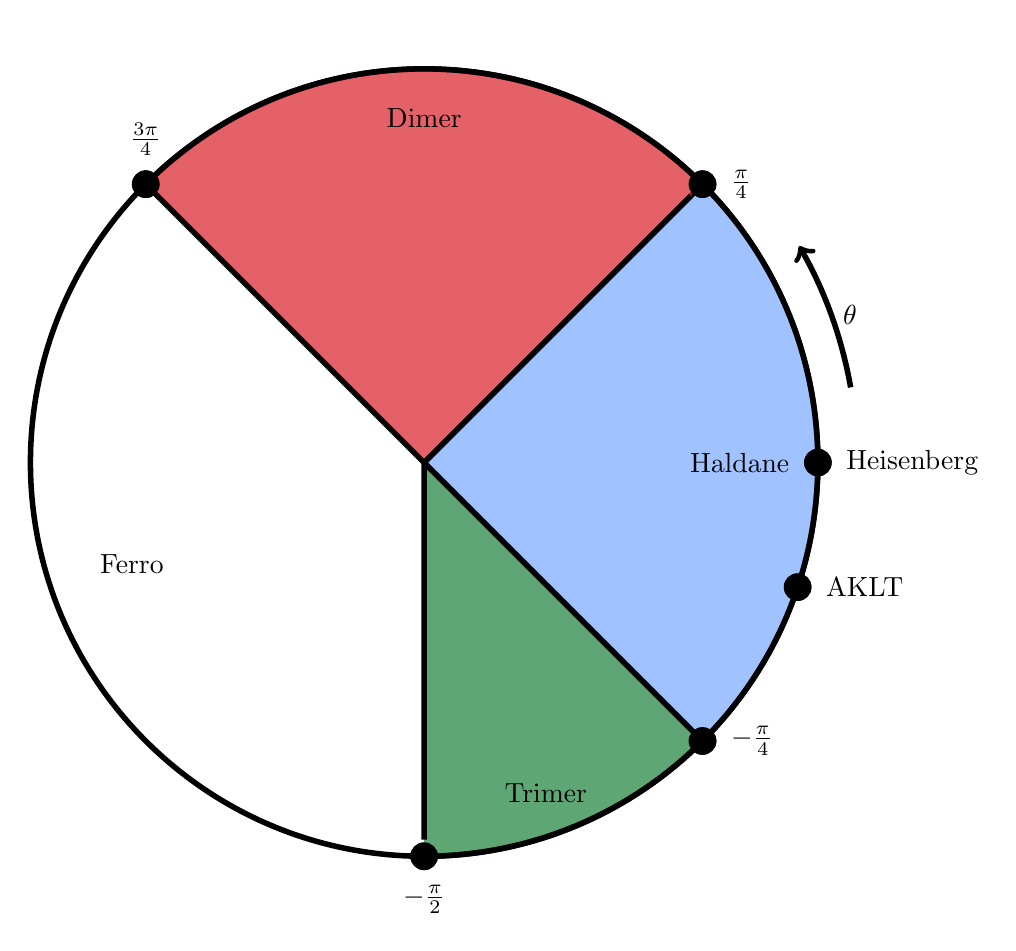
\begin{tikzpicture}[
        scale=5,
        font=\normalsize,
        dot/.style = {circle, inner sep=0pt, minimum size=10pt, fill=black},
        line width=2pt
    ]
    \node (A) at (45:1)  [dot, label=right:{$\frac{\pi}{4}$}] {};
    \node (C) at (-45:1) [dot, label=right:{$-\frac{\pi}{4}$}] {};
    \node (D) at (-90:1) [dot, label=below:{$-\frac{\pi}{2}$}] {};
    \node (E) at (135:1) [dot, label=above:{$\frac{3 \pi}{4}$}] {};
    \node (H) at (0:1)   [dot, label=right:Heisenberg] {};
    \node (K) at (-18.44:1) [dot, label=right:AKLT] {};

    \draw (0,0) circle [radius=1];

    \draw[fill=Blue40, fill opacity=0.7] (0,0) -- (C) arc (-45:45:1) -- (0,0);
    \draw[fill=Green, fill opacity=0.7] (0,0) -- (D) arc (-90:-45:1) -- (0,0);
    \draw[fill=Red, fill opacity=0.7] (0,0) -- (A) arc (45:135:1) -- (0,0);

    \node at (45:1)  [dot] {};
    \node at (-45:1) [dot] {};
    \node at (-90:1) [dot] {};
    \node at (135:1) [dot] {};
    \node at (0:1)   [dot] {};
    \node at (-18.44:1) [dot] {};

    \path (A) arc (45:135:1) node [below=10pt, midway] {Dimer};
    \path (C) arc (-45:45:1) node [left=6pt, midway] {Haldane};
    \path (D) arc (-90:-225:1) node [above right=10pt, midway] {Ferro};
    \path (C) arc (-45:-90:1) node [above=8pt, pos=0.6] {Trimer};

    \draw[->] (10:1.1) arc (10:30:1.1) node [midway, right] {$\theta$};
\end{tikzpicture}


        \end{tikzfigure}
    }

\end{columns}


\end{document}
